\documentclass[border=6pt,11pt]{standalone}
\usepackage{times}
\usepackage{amsmath,amssymb}
\usepackage{tikz}
\usetikzlibrary{arrows.meta, positioning, calc}
\begin{document}
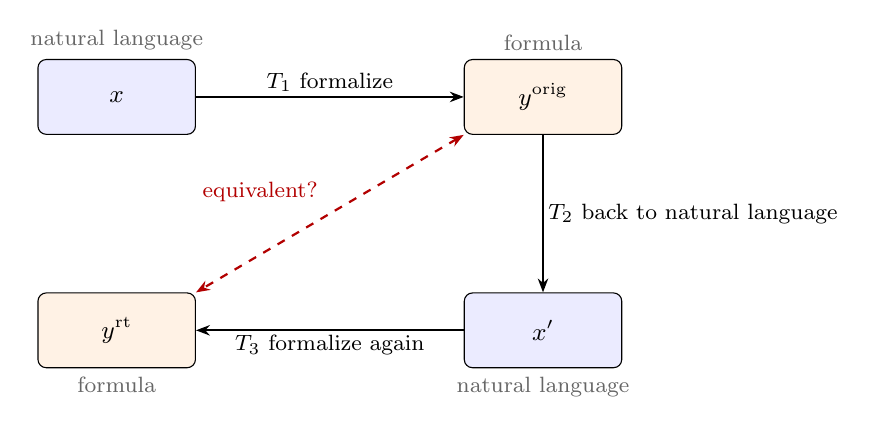
\begin{tikzpicture}[
    node distance=2.0cm and 3.4cm,
    box/.style={draw, rounded corners=3pt, minimum width=2.0cm, minimum height=0.95cm, align=center, font=\small},
    nlbox/.style={box, fill=blue!8},
    fmlbox/.style={box, fill=orange!10},
    arrow/.style={-{Stealth[length=5pt]}, thick},
    lbl/.style={font=\footnotesize, fill=white, inner sep=1.5pt},
    role/.style={font=\footnotesize, text=black!60, inner sep=1pt},
  ]
  \node[nlbox]  (x)  {$x$};
  \node[fmlbox, right=of x] (y) {$y^{\mathrm{orig}}$};
  \node[nlbox,  below=of y] (xp) {$x'$};
  \node[fmlbox, below=of x] (yrt) {$y^{\mathrm{rt}}$};

  \node[role, above=2pt of x]   {natural language};
  \node[role, above=2pt of y]   {formula};
  \node[role, below=2pt of xp]  {natural language};
  \node[role, below=2pt of yrt] {formula};

  \draw[arrow] (x)  -- node[lbl, above] {$T_1$ formalize} (y);
  \draw[arrow] (y)  -- node[lbl, right] {$T_2$ back to natural language} (xp);
  \draw[arrow] (xp) -- node[lbl, below] {$T_3$ formalize again} (yrt);

  \draw[{Stealth[length=5pt]}-{Stealth[length=5pt]}, dashed, thick, red!70!black]
    (y.south west) -- node[font=\footnotesize, text=red!70!black, above left=3pt and 3pt, inner sep=1pt]
    {equivalent?} (yrt.north east);
\end{tikzpicture}
\end{document}
